The distinct zones of cell beahviour observed in the roots of \emph{A. thaliana} play an essential role in maintaining optimal levels of growth. In this paper, we use recent research on brassinosteroids and the CLASP1 protein to develop two novel mathematical models of the zonation phenomenon. Our first model explains differences in behaviour in the epidermal cells of the wild type root of \emph{A thaliana} when compared two mutant roots in which elements of the CLASP1 signalling network have been perturbed. We find that length-based mechanism for cell division is sufficient to qualitatively explain the zonation patterns of these mutants. Then we present a model of a single cell in the wild type root fitted to levels of BR singalling levels and cell length from experimental observations. We discuss the benefits and drawbacks of this model and identify avenues for further study.

\medskip

\begin{figure}[!htbp]
    \centering
    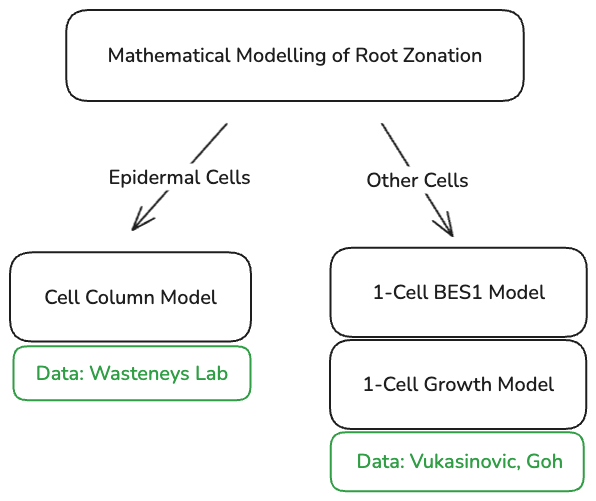
\includegraphics[width=10cm]{paper-overview.png}
    \label{fig:paper-overview}
    \caption{An overview of the models presented in this paper.}
\end{figure}
